\documentclass[12pt]{article}
\usepackage[spanish]{babel}
\usepackage{apacite}
\usepackage[utf8]{inputenc}
\usepackage{amsmath}
\usepackage{mathrsfs}
\usepackage{listings}
\usepackage[usenames]{color}
\definecolor{gray97}{gray}{.97}
\definecolor{gray75}{gray}{.75}
\definecolor{gray45}{gray}{.45}
\definecolor{azul1}{RGB}{141,198,163}
\definecolor{azul2}{RGB}{24,107,122}
\definecolor{verde1}{RGB}{44,186,34}
\usepackage{textcomp}
\lstset{
		frame=Ltb,
		framerule=1pt,
		framextopmargin=3pt,
		framexbottommargin=3pt,
		framexleftmargin=0.4cm,
		framesep=0pt,
		rulesep=.4pt,
		backgroundcolor=\color{gray97},
		rulesepcolor=,
        tabsize=4,
        rulecolor=\color{azul1},
        basicstyle=\scriptsize\rmfamily,
        upquote=true,
        aboveskip={1.5\baselineskip},
        columns=fixed,
        showstringspaces=false,
        extendedchars=true,
        breaklines=true,
        prebreak = \raisebox{0ex}[0ex][0ex]{\ensuremath{\hookleftarrow}},
        showtabs=false,
        showspaces=false,
        showstringspaces=false,
        identifierstyle=\rmfamily,
        keywordstyle=\color[rgb]{0,0,1},
        commentstyle=\color[rgb]{0.133,0.545,0.133},
        stringstyle=\color[rgb]{0.627,0.126,0.941},
        keywordstyle=\bfseries,
        %
		numbers=left,
		numbersep=15pt,
		numberstyle=\tiny,
		numberfirstline = false,
		breaklines=true,
		}
\usepackage{graphicx}
\usepackage[colorinlistoftodos]{todonotes}
\usepackage{natbib} %citas bibliograficas estilo APA :p
\usepackage{eso-pic}
\usepackage{avant}
\usepackage[top=2cm,bottom=2cm,left=2.5cm,right=3cm,headsep=8pt,a4paper]{geometry}
\usepackage{fancyhdr}
\pagestyle{fancy}
\fancyhf{}
%\fancyhead[LE,RO]{}
\fancyhead[RE,LO]{Control Digital y Aplicaciones}
\fancyfoot[CE,CO]{\rightmark}
\fancyfoot[LE,RO]{\thepage}
\renewcommand{\headrulewidth}{2pt}
\renewcommand{\footrulewidth}{1pt}
\usepackage{tabu}
\usepackage{array}
\usepackage{multirow}
\usepackage{amssymb}
\usepackage{makeidx}
\graphicspath{ {images/} }
\usepackage{wrapfig}
\usepackage{enumerate}
\usepackage{amsmath,tikz}
\usetikzlibrary{matrix}
\usepackage{steinmetz}
\newcommand*{\horzbar}{\rule[0.05ex]{2.5ex}{0.5pt}}
\usepackage{calc}
\date{\today}


\begin{document}

\begin{titlepage}
\newcommand{\HRule}{\rule{\linewidth}{0.5mm}} 
\center
\textsc{\LARGE  Benemérita Universidad \\[0.2cm] Autónoma de Puebla}\\[1.5cm] 

\includegraphics[width=4cm]{IMAGENES/escudo}\\[1cm]
\textsc{\Large Facultad de Ciencias de la Electrónica}\\[0.5cm] 
\textsc{\large Licenciatura en Electrónica}\\[0.5cm]
\HRule \\[0.4cm]
{ \huge \bfseries Tarea 1}\\[0.4cm] 
\HRule \\[1.5cm]
\begin{minipage}{\textwidth}
\center 

\emph{Profesor:} \\
Gutierres Arias Jose Eligio Moises, \\[1cm]
\vspace{10mm}
\begin{tabular}{ll}
\emph{Alumno:} & \emph{Número de Matrícula:}\\
Hanan Ronaldo Quispe Condori  & 555010653 \\
\end{tabular}
\end{minipage}\\[2cm]
%\today
\end{titlepage}

%\newpage
%~\vfill
%\thispagestyle{empty}
%\begin{figure}[hbtp]


%\includegraphics[width=4cm]{IMAGENES/motordc}
%\end{figure}
%\noindent \textsc{Trabajo Encargado: Problemas en MatLab \\ Máquinas Eléctricas \\ Universidad Nacional de San Antonio abad del Cusco}\\
%noindent \textsc{Ingeniería Electrónica }\\
%\noindent \textit{Tercera revisión, \today}

%\tableofcontents indice bloqueado xD

\newpage
\section{Transformada Z}
\subsection{Transformada Z Bilateral}
La transformada Z surge de la transformada de Fourier discreta, esta se define de la siguiente manera.
\begin{equation}
    \begin{split}
        %A&=J_{B}L(J_{p}+J_{1})\\
        \displaystyle\sum_{n=-\infty}^\infty\,x[n]e^{-j\omega n}\\
    \end{split}
    \label{eq:dft}
\end{equation}
Se tendrá la definición de la transformada Z tomando variable $z=re^{j\omega}$, bajo esta consideranción, la ecuación \ref{eq:dft} quedara de la siguiente forma, tomemos en cuenta que cuando $r=1$ la transformada Z será la transformada de Fourier discreta (\cite{schafer1989discrete}).
\begin{equation}
    \begin{split}
        \displaystyle\sum_{n=-\infty}^\infty\,x[n]z^{-n}\\
    \end{split}
    \label{eq:zt}
\end{equation}
Tomaremos una nueva notación para ecuación \ref{eq:zt} 
\begin{equation}
    \begin{split}
        \mathscr{Z}\{x[n]\}&=\displaystyle\sum_{n=-\infty}^\infty\,x[n]z^{-n}=X(z)\\
    \end{split}
    \label{eq:zt1}
\end{equation}
La sumatoria \ref{eq:zt} convergerá solo si se cumple que
\begin{equation}
    \begin{split}
        \displaystyle\sum_{n=-\infty}^\infty\,|x[n]||z^{-n}|<\infty\\
        \displaystyle\sum_{n=-\infty}^\infty\,|x[n]||(re)^{-j\omega n}|<\infty\\
        \displaystyle\sum_{n=-\infty}^\infty\,|x[n]r^{-n}|<\infty\\
    \end{split}
    \label{eq:zt2}
\end{equation}
Para que la ecuación \ref{eq:zt2} se cumpla la secuencia debe ser absolutamente sumable, debemos encontrar el rango de valores de $r$ para que esto se cumpla, con este objeto, procederemos a operar en \ref{eq:zt2} como sigue.
\begin{equation}
    \begin{split}
        X(z)&\leq\displaystyle\sum_{n=-\infty}^{-1}\,|x(n)r^{-n}|+\displaystyle\sum_{n=0}^\infty\,|x(n)r^{-n}|\\
        X(z)&\leq\displaystyle\sum_{n=}^\infty\,|x(-n)r^{n}|+\displaystyle\sum_{n=0}^\infty\,|x(n)r^{-n}|\\
    \end{split}
    \label{eq:zt3}
\end{equation}
De \ref{eq:zt3} podemos sacar las siguientes relaciones para $n$, $1\leq n<\infty$ y $0\leq n<\infty$, estas relaciones nos daran una region donde la transformada Z convergerá, si analizamos esta region, se podrá obtener información sobre la secuencia
\begin{itemize}
    \item Secuencia de longitud finita $0<|z|<\infty$
    \item Secuencia limitada por la derecha $R_{x-}<|z|<\infty$
    \item Secuencia limitada por la izquierda $0<|z|<R_{x+}$
    \item Secuencia bilateral $R_{x-}<|z|<R_{x+}$     
\end{itemize}
\subsubsection{Propiedades de la Transformada Z}
\textbf{Linealidad}
\vspace{5mm}

%\setlength{\parindent}{10ex}
Esta propiedad establece que\par

\begin{equation}
    \begin{split}
        \displaystyle\sum_{n=-\infty}^{\infty}\,(ax_{1}[n]+bx_{2}[n])z^{-n}&=a\displaystyle\sum_{n=-\infty}^{\infty}\,x_{1}[n]z^{-n}+b\displaystyle\sum_{n=-\infty}^{\infty}\,x_{2}[n]z^{-n}\\
    \end{split}
    \label{eq:lineal}
\end{equation}

\textbf{Desplazamiento en el Tiempo}
\vspace{5mm}

%\setlength{\parindent}{10ex}
Esta propiedad establece que\par

\begin{equation}
    \begin{split}
        x[n-n_{0}]\xrightarrow{\mathscr{Z}}z^{-n_{0}}X(z)\\
    \end{split}
    \label{eq:despla_time}
\end{equation}

Demostración
\begin{equation}
    \begin{split}
        X(Z)&=\displaystyle\sum_{n=-\infty}^{\infty}\,x[n-n_{0}]z^{-n}\\
    \end{split}
    \label{eq:despla_time1}
\end{equation}

Haciendo cambio de variable $m=n-n_{0}$ en \ref{eq:despla_time1} se tendrá
\begin{equation}
    \begin{split}
        Y(Z)&=\displaystyle\sum_{n=-\infty}^{\infty}\,x[m]z^{m+n_{0}}\\
        Y(Z)&=z^{-m_{0}}X(Z)\\
    \end{split}
    \label{eq:despla_time2}
\end{equation}

\textbf{Multiplicación por una Secuencia Exponencial}
\vspace{5mm}

%\setlength{\parindent}{10ex}
Esta propiedad establece que\par

\begin{equation}
    \begin{split}
        z^n_{0}x[n]\xrightarrow{\mathscr{Z}}X(z/z_{0})\\
    \end{split}
    \label{eq:multi}
\end{equation}

Demostración
\begin{equation}
    \begin{split}
        X(Z)&=\displaystyle\sum_{n=-\infty}^{\infty}\,(z^n_{0}x[n])z^{-n}\\
        X(Z)&=\displaystyle\sum_{n=-\infty}^{\infty}\,x[n](\frac{z}{z_{0}})^{-n}\\
    \end{split}
    \label{eq:multipli1}
\end{equation}
De \ref{eq:multipli1} podemos ver que se cumple \ref{eq:multi}

\textbf{Propiedad de Convolución}
\vspace{5mm}

%\setlength{\parindent}{10ex}
La convolución de dos secuencias, equivale a la multiplicación de sus respectivas transformadas Z.\par
\begin{equation}
    \begin{split}
        x_{1}[n]*x_{2}[n]\xrightarrow{\mathscr{Z}}X_{1}(Z)X_{2}(Z)\\
    \end{split}
    \label{eq:convolu}
\end{equation}
Demostración

Sea la convolución de $x_{1}[n],x_{2}[n]$ en tiempo discreto
\begin{equation}
    \begin{split}
        y[n]=\displaystyle\sum_{k=-\infty}^{\infty}\,x_{1}[k]x_{2}[n-k]\\
    \end{split}
    \label{eq:convolu_demo}
\end{equation}
Calculando la transformada Z de la ecuación \ref{eq:convolu_demo} se tendrá.
\begin{equation}
    \begin{split}
        Y(Z)=\displaystyle\sum_{n=-\infty}^{\infty}\,(\displaystyle\sum_{k=-\infty}^{\infty}\,x_{1}[k]x_{2}[n-k])z^{-n}\\
    \end{split}
    \label{eq:convolu_demo1}
\end{equation}
Haciendo cambio de variable $m=n-k$ e intercambiando el orden de la suma se tendrá
\begin{equation}
    \begin{split}
        Y(Z)&=\displaystyle\sum_{k=-\infty}^{\infty}\,x_{1}[k](\displaystyle\sum_{m=-\infty}^{\infty}\,x_{2}[m]z^{-m})z^{-k}\\
        Y(Z)&=(\displaystyle\sum_{k=-\infty}^{\infty}\,x_{1}[k]z^{-k})X_{2}(Z)\\
        Y(Z)&=X_{1}(Z)X_{2}(Z)\\
    \end{split}
    \label{eq:convolu_demo2}
\end{equation}

\textbf{Diferenciación}
\vspace{5mm}

%\setlength{\parindent}{10ex}
Esta propiedad estipula que\par
\begin{equation}
    \begin{split}
        nx_{1}[n]\xrightarrow{\mathscr{Z}}-z\frac{dX(z)}{dz}\\
    \end{split}
    \label{eq:dif}
\end{equation}
Demostración
Sea la transformada Z de la secuencia $x[n]$ 
\begin{equation}
    \begin{split}
        Y(Z)=\displaystyle\sum_{n=-\infty}^{\infty}\,x[n]z^{-n}\\
    \end{split}
    \label{eq:dif_demo}
\end{equation}
Derivando la ecuación \ref{eq:dif_demo} con respecto a $z$ y multiplicando por $-z$
\begin{equation}
    \begin{split}
        -z\frac{dX(z)}{dz}&=-z\displaystyle\sum_{n=-\infty}^{\infty}\,(-n)x[n]z^{-n-1}\\
        -z\frac{dX(z)}{dz}&=\displaystyle\sum_{n=-\infty}^{\infty}\,nx[n]z^{-n}\\
    \end{split}
    \label{eq:dif_demo1}
\end{equation}
\subsection{Transformada Z Unilateral}
La transformada bilateral necesita ser definida para el rango completo de $-\infty<n<\infty$, este requerimiento impide que sea usada para la resolución de problemas, los sistemas descritos por ecuaciones de diferencias con condiciones iniciales diferentes a cero, esto ya que la entrada aplicada en un tiempo finito $n_{0}$ esta especificada para $n\ge n_{0}$, pero no necesariamente será cero para $n\le n_{0}$, por lo que la transformada bilateral no puede ser usada; para solucionar este problema, se tendrá que definir la transformada Z unilateral. \cite{proakis1996digital}
\begin{equation}
    \begin{split}
        X^+(z)&=\displaystyle\sum_{n=0}^{\infty}\,x[n]z^{-n}\\
    \end{split}
    \label{eq:zt_unilateral}
\end{equation}
La notación antes usada para la transformada Z cambiara a $\mathscr{Z}^+\{x[n]\}$, esta transformada difiere de la transformada bilateral en el límite inferior de la sumatoria, el cual es siempre cero.

Casi todas las propiedades estudidadas para la transformada bilateral se cumplen tambien para la transformada unilateral, a excepción de la propiedad de desplazamiento en el tiempo.

\textbf{Retardo en el Tiempo}
\vspace{5mm}

Sea 
\begin{equation}
    \begin{split}
        x[n]\xrightarrow{\mathscr{Z}^+}X^+(z)\\
    \end{split}
    \label{eq:uzt_delay}
\end{equation}

Sabemos que $x[n]$ será causal entonces se tendrá

\begin{equation}
    \begin{split}
        \mathscr{Z}^+\{x[n-k]\}&=z^{-k}[\displaystyle\sum_{l=-k}^{-1}\,x[l]z^{-l}+\displaystyle\sum_{l=0}^{\infty}\,x[l]z^{-l}]\\
        \mathscr{Z}^+\{x[n-k]\}&=z^{-k}[\displaystyle\sum_{l=-1}^{-k}\,x[l]z^{-l}+X^+(z)]\\
    \end{split}
    \label{eq:uzt_delay1}
\end{equation}
Haciendo el cambio de variable $n=-l$ se tendrá
\begin{equation}
    \begin{split}
        \mathscr{Z}^+\{x[n-k]\}&=z^{-k}[\displaystyle\sum_{n=1}^{k}\,x[-n]z^{n}+X^+(z)], \quad k>0\\
    \end{split}
    \label{eq:uzt_delay2}
\end{equation}

\textbf{Adelanto en el Tiempo}
\vspace{5mm}

Sea 
\begin{equation}
    \begin{split}
        x[n]\xrightarrow{\mathscr{Z}^+}X^+(z)\\
    \end{split}
    \label{eq:uzt_advance}
\end{equation}

Sabemos que $x[n]$ será causal entonces se tendrá

\begin{equation}
    \begin{split}
        \mathscr{Z}^+\{x[n+k]\}&=z^{-k}\displaystyle\sum_{n=0}^{\infty}\,x[n+k]z^{-n}=z^{k}\displaystyle\sum_{l=k}^{\infty}\,x[l]z^{-l}\\
    \end{split}
    \label{eq:uzt_advance1}
\end{equation}
Haciendo el cambio de variable $n=k-l$ se tendrá
\begin{equation}
    \begin{split}
        X^+(z)&=\displaystyle\sum_{l=0}^{k-1}\,x[l]z^{-l}+\displaystyle\sum_{l=k}^{\infty}\,x[l]z^{-l}\\
    \end{split}
    \label{eq:uzt_advance2}
\end{equation}
Combinando la ecuación \ref{eq:uzt_advance2} obtendremos finalmente
\begin{equation}
    \begin{split}
        \mathscr{Z}^+\{x[n+k]\}&=z^{k}[X^+(z)-\displaystyle\sum_{n=0}^{k-1}\,x[n]z^{-n}], \quad k>0\\
    \end{split}
    \label{eq:uzt_advance3}
\end{equation}
\subsubsection{Transformada Z de Funciones Elementales}

\textbf{Escalon Unitario}
\vspace{5mm}

Sea $x[n]=\mu(n)$

\vspace{5mm}
Usando la definición de la transformada Z unilateral y operando se tendrá.

\begin{equation}
    \begin{split}
        X^+(z)&=\displaystyle\sum_{n=0}^{\infty}\,\mu(n)z^{-n}\\
        X^+(z)&=\displaystyle\sum_{n=0}^{\infty}\,z^{-n}\\
    \end{split}
    \label{eq:ejer1}
\end{equation}

Sabemos que la sumatoria \ref{eq:ejer1} es una serie geométrica cuya fórmula general es
\begin{equation}
    \begin{split}
        \displaystyle\sum_{n=0}^{\infty}\,a_{n}r^{n}&=\frac{a}{1-r}\\
    \end{split}
    \label{eq:ejer11}
\end{equation}

De \ref{eq:ejer11} se tendrá finalmente que 
\begin{equation}
    \begin{split}
        X^+(z)&=\displaystyle\sum_{n=0}^{\infty}\,z^{-n}=\frac{1}{1-z^{-1}}\\
    \end{split}
    \label{eq:ejer12}
\end{equation}

\textbf{Rampa Unitaria}
\vspace{5mm}

Sea $x[n]=n$
Usando la definición de la transformada Z unilateral y operando se tendrá.

\begin{equation}
    \begin{split}
        X^+(z)&=\displaystyle\sum_{n=0}^{\infty}\,nz^{-n}\\
    \end{split}
    \label{eq:ejer2}
\end{equation}

Expandiendo la sumatoria tendremos que  
\begin{equation}
    \begin{split}
        \displaystyle\sum_{n=0}^{\infty}\,nz^{-n}&=z^{-1}+2z^{-2}+3z^{-3}+...+nz^{-n}\\
    \end{split}
    \label{eq:ejer21}
\end{equation}

Multiplicando \ref{eq:ejer21} por $-2z^{-1}$
\begin{equation}
    \begin{split}
        -2z^{-1}\displaystyle\sum_{n=0}^{\infty}\,nz^{-n}&=z^{-1}+2z^{-2}+3z^{-3}+...+nz^{-n}\\
    \end{split}
    \label{eq:ejer22}
\end{equation}

Sumando \ref{eq:ejer21} y \ref{eq:ejer22} se tendrá 
\begin{equation}
    \begin{split}
        \displaystyle\sum_{n=0}^{\infty}\,nz^{-n}&=\frac{z^{-1}-2nz^{-(n+1)}+nz^{-(n+2)}}{(1-z^{-1})^2}\\
    \end{split}
    \label{eq:ejer23}
\end{equation}

Llevando el límite cuando n tiende a $\infty$ en \ref{eq:ejer23} se tendrá finalmente.
\begin{equation}
    \begin{split}
        X^+(z)&=\displaystyle\sum_{n=0}^{\infty}\,nz^{-n}=\frac{z^{-1}}{(1-z^{-1})^2}\\
    \end{split}
    \label{eq:ejer24}
\end{equation}

\textbf{Función Polinomial}
\vspace{5mm} 

Sea $x[n]=a^n$

\vspace{5mm}
Usando la definición de la transformada Z unilateral y operando se tendrá.
\begin{equation}
    \begin{split}
        X^+(z)&=\displaystyle\sum_{n=0}^{\infty}\,a^nz^{-n}\\
        X^+(z)&=\displaystyle\sum_{n=0}^{\infty}\,(az^{-1})^{n}\\
    \end{split}
    \label{eq:ejer3}
\end{equation}

Tendremos que \ref{eq:ejer3} tiene la misma forma que \ref{eq:ejer11}, por lo que podemos dar una respuesta directamente.
\begin{equation}
    \begin{split}
        X^+(z)&=\displaystyle\sum_{n=0}^{\infty}\,a^nz^{-n}=\frac{1}{1-az^{-1}}\\
    \end{split}
    \label{eq:ejer31}
\end{equation}

\textbf{Función Exponencial}
\vspace{5mm} 

Sea $x[n]=e^{-an}$

\vspace{5mm}
Usando la definición de la transformada Z unilateral y operando se tendrá.
\begin{equation}
    \begin{split}
        X^+(z)&=\displaystyle\sum_{n=0}^{\infty}\,e^{-an}z^{-n}\\
        X^+(z)&=\displaystyle\sum_{n=0}^{\infty}\,(e^{-a}z^{-1})^{n}\\
    \end{split}
    \label{eq:ejer4}
\end{equation}

Tendremos que \ref{eq:ejer4} tiene la misma forma que \ref{eq:ejer11}, por lo que podemos dar una respuesta directamente.
\begin{equation}
    \begin{split}
        X^+(z)&=\displaystyle\sum_{n=0}^{\infty}\,e^{-an}z^{-n}=\frac{1}{1-e^{-a}z^{-1}}\\
    \end{split}
    \label{eq:ejer41}
\end{equation}

\textbf{Función Senoidal}
\vspace{5mm} 

La identidad de Euler establece que $sen(\omega n)=\frac{e^{i\omega n}-e^{-i\omega n}}{2i}$

\vspace{5mm}
Usando la definición de la transformada Z unilateral y usando la propiedad de linealidad se tendrá.
\begin{equation}
    \begin{split}
        X^+(z)&=\displaystyle\sum_{n=0}^{\infty}\,(\frac{e^{iwn}-e^{-iwn}}{2i})z^{-n}\\
        X^+(z)&=\frac{1}{2i}\displaystyle\sum_{n=0}^{\infty}\,e^{iwn}z^{-n}-\frac{1}{2i}\displaystyle\sum_{n=0}^{\infty}\,e^{-iwn}z^{-n}\\
        X^+(z)&=\frac{1}{2i}(\displaystyle\sum_{n=0}^{\infty}\,e^{iwn}z^{-n}-\displaystyle\sum_{n=0}^{\infty}\,e^{-iwn}z^{-n})\\
    \end{split}
    \label{eq:ejer5}
\end{equation}

Tendremos que \ref{eq:ejer5} tiene la misma forma que \ref{eq:ejer11}, por lo que, operando se tendrá.
\begin{equation}
    \begin{split}
        X^+(z)&=\frac{1}{2i}(\frac{1}{1-z^{-1}e^{i\omega}}-\frac{1}{1-z^{-1}e^{-i\omega}})\\
        X^+(z)&=\frac{z^{-1}sen(\omega)}{1+z^{-2}-2z^{-1}cos(\omega)}\\
    \end{split}
    \label{eq:ejer51}
\end{equation}

Para función coseno se tendrá que 
a identidad de Euler establece que $cos(\omega n)=\frac{e^{i\omega n}+e^{-i\omega n}}{2}$

\vspace{5mm}
Usando la definición de la transformada Z unilateral y la propiedad de linealidad se tendrá.
\begin{equation}
    \begin{split}
        X^+(z)&=\displaystyle\sum_{n=0}^{\infty}\,(\frac{e^{i\omega n}+e^{-i\omega n}}{2})z^{-n}\\
        X^+(z)&=\frac{1}{2}\displaystyle\sum_{n=0}^{\infty}\,e^{iwn}z^{-n}+\frac{1}{2}\displaystyle\sum_{n=0}^{\infty}\,e^{-iwn}z^{-n}\\
        X^+(z)&=\frac{1}{2}(\displaystyle\sum_{n=0}^{\infty}\,e^{iwn}z^{-n}+\displaystyle\sum_{n=0}^{\infty}\,e^{-iwn}z^{-n})\\
    \end{split}
    \label{eq:ejer6}
\end{equation}

Tendremos que \ref{eq:ejer6} tiene la misma forma que \ref{eq:ejer11}, por lo que, operando se tendrá.
\begin{equation}
    \begin{split}
        X^+(z)&=\frac{1}{2}(\frac{1}{1-z^{-1}e^{i\omega}}+\frac{1}{1-z^{-1}e^{-i\omega}})\\
        X^+(z)&=\frac{1-z^{-1}cos(\omega)}{1+z^{-2}-2z^{-1}cos(\omega)}\\
    \end{split}
    \label{eq:ejer61}
\end{equation}

\subsection{Ejemplos}

\begin{itemize}
    \item \textbf{$e^{-at}sen(\omega t)$}
    \vspace{5mm}

Sea su representación en tiempo discreto $x[n]=e^{-aTn}sen(\omega Tn)$, usaremos la propiedad de multiplicación por una secuencia exponencial para su resolución.

De \ref{eq:ejer51} sabemos que 
\begin{equation}
    \begin{split}
        X^+(z)&=\frac{z^{-1}sen(\omega T)}{1+z^{-2}-2z^{-1}cos(\omega T)}\\
        X^+(\frac{z}{e^{-aT}})&=\frac{(\frac{z}{e^{-aT}})^{-1}sen(\omega T)}{1+(\frac{z}{e^{-aT}})^{-2}-2(\frac{z}{e^{-aT}})^{-1}cos(\omega T)}\\
        X^+(\frac{z}{e^{-aT}})&=\frac{e^{-aT}z^{-1}sen(\omega T)}{1+e^{-2aT}z^{-2}-2z^{-1}e^{-aT}cos(\omega T)}\\
    \end{split}
    \label{eq:ejer62}
\end{equation}

\item \textbf{$e^{-at}cos(\omega t)$}
    \vspace{5mm}

Sea su representación en tiempo discreto $x[n]=e^{-aTn}cos(\omega Tn)$, usaremos la propiedad de multiplicación por una secuencia exponencial para su resolución.

De \ref{eq:ejer61} sabemos que 
\begin{equation}
    \begin{split}
        X^+(z)&=\frac{1-z^{-1}cos(\omega T)}{1+z^{-2}-2z^{-1}cos(\omega T)}\\
        X^+(\frac{z}{e^{-aT}})&=\frac{1-(\frac{z}{e^{-aT}})^{-1}cos(\omega T)}{1+(\frac{z}{e^{-aT}})^{-2}-2(\frac{z}{e^{-aT}})^{-1}cos(\omega T)}\\
        X^+(\frac{z}{e^{-aT}})&=\frac{1-e^{-aT}z^{-1}cos(\omega T)}{1+e^{-2aT}z^{-2}-2e^{-aT}z^{-1}cos(\omega T)}\\
    \end{split}
    \label{eq:ejer72}
\end{equation}

\item \textbf{$x[n]=\frac{-1}{n}(\frac{1}{2})^n$}
    \vspace{5mm}

    Usaremos la propiedad de la diferenciación para resolver este problema, para ello procederemos como sigue.
    \begin{equation}
        \begin{split}
            nx[n]&=-(\frac{1}{2})^n\\
            \mathscr{Z}\{nx[n]\}&=-z\frac{dX(z)}{dz}\\
            -z\frac{dX(z)}{dz}&=\frac{-1}{1-\frac{1}{2}z^{-1}}\\
            \frac{dX(z)}{dz}&=\frac{-2}{1-2z}\\
            X(z)&=log(1-2z)\\
        \end{split}
        \label{eq:ejer8}
    \end{equation}
    
\item \textbf{$x[n]=2(\frac{1}{2})^n-(\frac{1}{4})^n$}
    \vspace{5mm}

    Por la naturaleza de la secuencia tendremos
    \begin{equation}
        \begin{split}
            X(z)&=\frac{-1}{1-\frac{1}{4}z^{-1}}+\frac{2}{1-\frac{1}{2}z^{-1}}\\
            X(z)&=\frac{1}{(1-\frac{1}{4}z^{-1})(1-\frac{1}{2}z^{-1})}\\
        \end{split}
        \label{eq:ejer9}
    \end{equation}


\item \textbf{Sean las secuencias $x_{1}[n]=\delta[n]+2\delta[n-1]+\delta[n-2],x_{2}[n]=\delta[n]-\delta[n-1]$ calcular $\mathscr{Z}(x_{1}[n]*x_{2}[n])$}
    \vspace{5mm}

    Usaremos la propiedad de la convolución para resolver este problema
    \begin{equation}
        \begin{split}
            X_{1}(z)&=1+2z^{-1}+z^{-2}\\
            X_{2}(z)&=1-z^{-1}\\
            X(z)&=X_{1}(z)X_{2}(z)\\
            X(z)&=1+z^{-1}-z^{-2}-z^{-3}\\
        \end{split}
        \label{eq:ejerlast}
    \end{equation}
\end{itemize}
\section{Función de Transferencia}
La función de transferencia de un sistema lineal se define como el cociente de la transformada de Laplace de la variable de salida y la transformada de Laplace de la variable de entrada, todo esto con condiciones iniciales igual a cero.
Esta relación describe la dinámica del sistema a considerar; una función de transferencia debe ser definida solo para sistemas lineales, estacionarios. Un sistema no estacionario(variante en el tiempo) tiene más de una variable que varia en el tiempo y la transformada de Laplace no debe ser usada. Una función de transferencia da una descripción de la entrada y salida del sistema, pero no incluye ninguna información con respecto a la estructura interna del sistema ni su comportamiento.\cite{dorf2005sistemas}

\vspace{5mm}
El proceso parte de las ecuaciones diferenciales que modelan el sistema, se usa la transformada de Laplace y se calcula el cociente $\frac{salida}{entrada}$ en función de la variable de Laplace $s$

\subsection{Ejemplos}
\begin{itemize}
    \item Hallar la función de transferencia del sistema mostrado en la figura
    \begin{figure}[h]
        \centering
            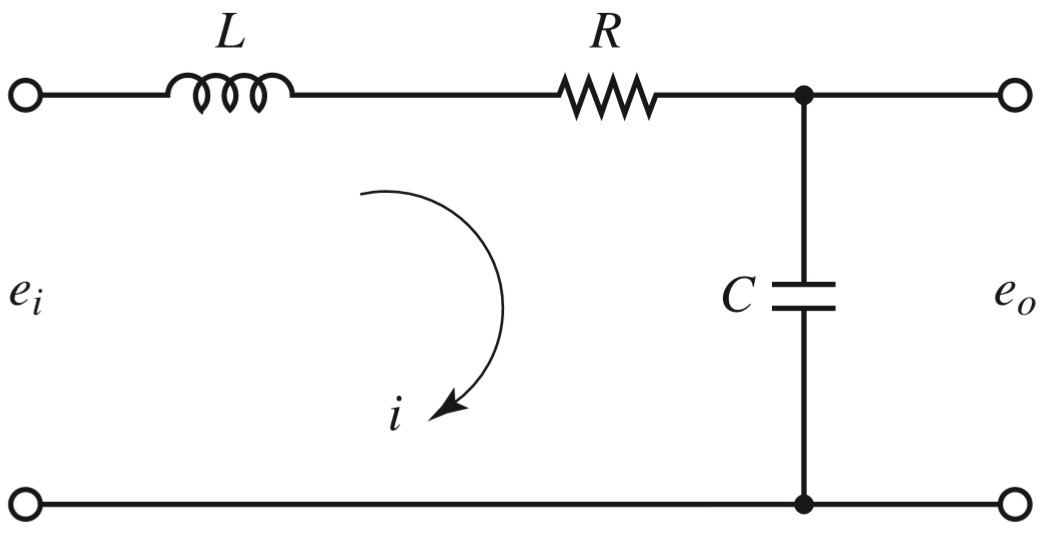
\includegraphics[width=5cm]{IMAGENES/transfer1}
            \caption{LRC en serie.}
    \end{figure}
    Usando KLV en el circuito mostrado se tendran las siguientes ecuaciones 
    \begin{equation}
        \begin{split}
            e_{i}&=L\frac{di}{dt}+Ri+\frac{1}{C}\int i dt\\
            e_{o}&=\frac{1}{C}\int i dt\\
        \end{split}
        \label{eq:ejer_transfer1}
    \end{equation}
    Usando la transformada de Laplace en \ref{eq:ejer_transfer1} se tendrá
    \begin{equation}
        \begin{split}
            E_{i}(s)&=LsI(s)+RI(s)+\frac{1}{C}\frac{1}{s}I(s)\\
            E_{o}(s)&=\frac{1}{C}\frac{1}{s}I(s)\\
        \end{split}
        \label{eq:ejer_transfer11}
    \end{equation}
    De \ref{eq:ejer_transfer11} se podrá facilmente calcular
    \begin{equation}
    \begin{split}
        \frac{E_{o}(s)}{E_{i}(s)}&=\frac{1}{LCs^2+RCs+1}\\
    \end{split}
    \label{eq:ejer_transfer12}
    \end{equation}

    \item Hallar la función de transferencia del sistema mostrado en la figura
    %\vspace{50mm}
    \begin{figure}[h]
        \centering
            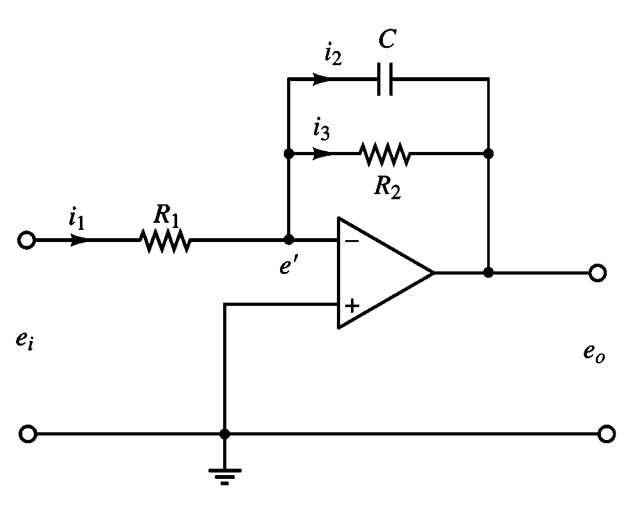
\includegraphics[width=4cm]{IMAGENES/transfer2}
            \caption{Op-amp ideal.}
    \end{figure}
    Usando KCL en el circuito dado se tendrá lo siguiente 
    \begin{equation}
        \begin{split}
            i_{1}&=\frac{e_{i}-e'}{R_{1}}\\
            i_{2}&=C\frac{d(e'-e_{o})}{dt}\\
            i_{3}&=\frac{e'-e_{o}}{R_{2}}\\
            i_{1}&=i_{2}+i_{3}\\
            \frac{e_{i}-e'}{R_{1}}&=C\frac{d(e'-e_{o})}{dt}+\frac{e'-e_{o}}{R_{2}}\\
        \end{split}
        \label{eq:ejer_transfer2}
    \end{equation}
    Usando la transformada de Laplace en \ref{eq:ejer_transfer2} se tendrá.
    \begin{equation}
        \begin{split}
            \frac{E_{i}}{R_{1}}&=-\frac{R_{2}Cs+1}{R_{2}}\\
        \end{split}
        \label{eq:ejer_transfer21}
    \end{equation}
    De \ref{eq:ejer_transfer21} se podrá calcular
    \begin{equation}
        \begin{split}
        \frac{E_{o}(s)}{E_{i}(s)}&=-\frac{R_{2}}{R_{1}}\frac{1}{R_{2}Cs+1}\\
        \end{split}
    \label{eq:ejer_transfer22}
    \end{equation}

    \item  Hallar la función de transferencia $\frac{Y(s)}{U(s)}$ del sistema mostrado en la figura
    \begin{figure}[h]
        \centering
            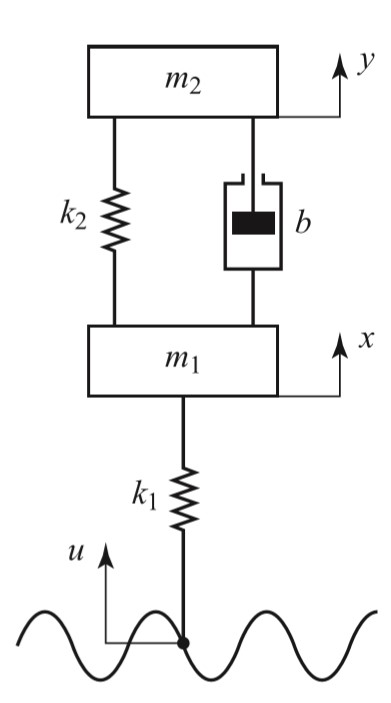
\includegraphics[width=4cm]{IMAGENES/transfer3}
            \caption{Sistema mecánico.}
    \end{figure}
    Las ecuaciones apartir de la segunda ley de Newton serán.
    \begin{equation}
        \begin{split}
        m_{1}\ddot{x}&=k_{2}(y-x)+b(\dot{y}-\dot{x})+k_{1}(u-x)\\
        m_{2}\ddot{y}&=-k_{2}(y-x)-b(\dot{y}-\dot{x})\\
        \end{split}
    \label{eq:ejer_transfer3}
    \end{equation}
    Usando la transformada de Laplace en \ref{eq:ejer_transfer3}
    \begin{equation}
        \begin{split}
            X(s)(m_{1}s^2+bs+k_{1}+k_{2})&=Y(s)(bs+k_{2})+k_{1}U(s)\\
        \end{split}
        \label{eq:ejer_transfer31}
    \end{equation}
    Por condición de la función de transferencia $U(s)=0$, ordenando tendremos la función de transferencia.
    \begin{equation}
        \begin{split}
        \frac{Y(s)}{U(s)}&=\frac{k_{1}(bs+k_{2})}{m_{1}m_{2}s^4+(m_{1}+m_{2})bs^3+[k_{1}m_{2}+(m_{1}+m_{2})k_{2}]s^2+k_{1}bs+k_{1}k_{2}}\\
        \end{split}
    \label{eq:ejer_transfer32}
    \end{equation}

    \item Hallar la función de transferencia del sistema mostrado en la figura
    \begin{figure}[h]
        \centering
            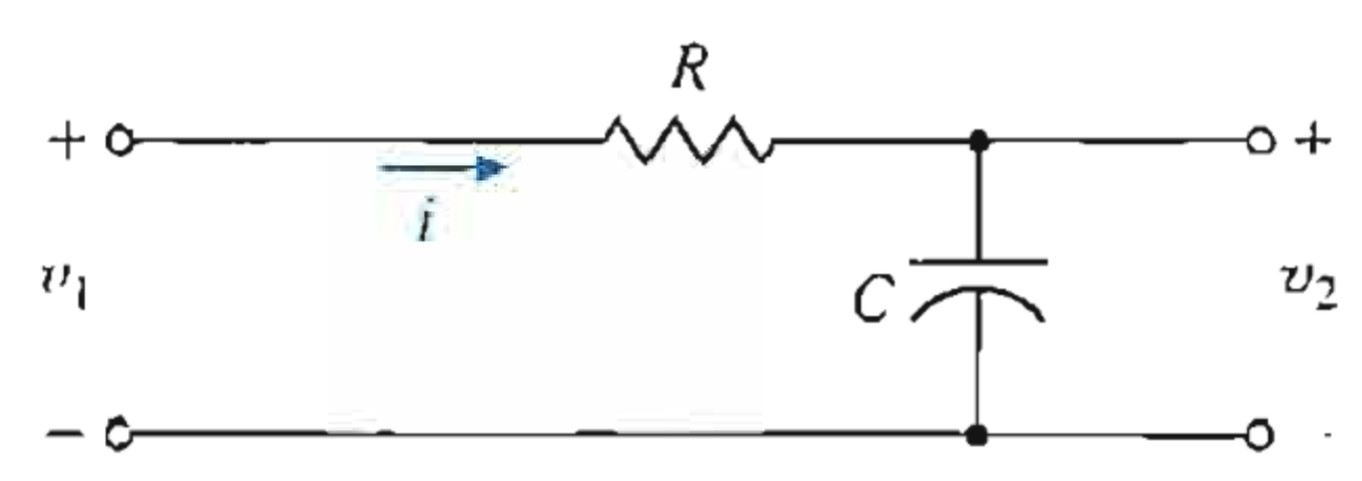
\includegraphics[width=5cm]{IMAGENES/transfer4}
            \caption{Circuito RC en Serie.}
    \end{figure}

    Usando KVL en la red se tiene
    \begin{equation}
        \begin{split}
        v_{1}(t)&=i(t)R+\frac{1}{C}\int idt\\
        v_{2}(t)&=\frac{1}{C}\int idt\\
        \end{split}
    \label{eq:ejer_transfer4}
    \end{equation}
    Llevando al dominio de Laplace se tiene
    \begin{equation}
        \begin{split}
        V_{1}(s)&=I(s)(R+\frac{1}{Cs})\\
        V_{2}(s)&=I(s)\frac{1}{Cs}\\
        \end{split}
    \label{eq:ejer_transfer41}
    \end{equation}
    Finalmente
    \begin{equation}
        \begin{split}
        \frac{V_{2}(s)}{V_{1}(s)}&=\frac{1}{sRC+1}\\
        \end{split}
    \label{eq:ejer_transfer42}
    \end{equation}
\end{itemize}

\section{Representación en Variables de Estado}
El estado de un sistema en un instante dado, es el valor de unas variables internas del sistema(en ocaciones ficticias y no accesibles) que describen la evolución del mismo a lo largo del tiempo.

\textbf{Estado:}
\vspace{5mm}
El estado de un sistema dinámico en cualquier instante de tiempo $t_{0}$ es el conjunto más pequeño de números suficiente para determinar el comportamiento o disposición del sistema para todo tiempo $t\geq t_{0}$.

\vspace{5mm}
\textbf{Variable de Estado:}
\vspace{5mm}

Se llama al conjunto linealmente independiente de variables que se utilizan para especificar el estado de un sistema.

Se dice que un conjunto de $n$ variables $x_{1},x_{2},x_{3},...,x_{n}$ es linealmente independiente si no existe un conjunto de constantes $c_{1},c_{2},c_{3},...,c_{n}$ que sean todas cero, que satisfagan lo siguiente

\begin{equation}
    \begin{split}
        c_{1}x_{1}+c_{2}x_{2}+c_{3}x_{3}+...+c_{n}x_{n}=0
    \end{split}
    \label{eq:lin_indepen}
\end{equation}

\textbf{Ecuación de Estado:}
\vspace{5mm}

Las variables de estado deben formularse de tal modo que si uno de conoce sus cariables en un instante dado, junto con los valores de las variables de entrada para este momento y para todo momento futuro, entonces la disposición del sistema y estas variables se determinan completamente para ese momento y para cualquier momento futuro.
\begin{equation}
    \begin{split}
        \frac{dx_{1}}{dt}&=f_{1}(x_{1},x_{2},...,x_{n},u_{1},u_{2},...,u_{n}) \quad x_{1}(t_{0})={x_{1}}_{t-0}\\
        \frac{dx_{2}}{dt}&=f_{2}(x_{1},x_{2},...,x_{n},u_{1},u_{2},...,u_{n}) \quad x_{2}(t_{0})={x_{2}}_{t-0}\\
        _:^:\\
        \frac{dx_{n}}{dt}&=f_{n}(x_{1},x_{2},...,x_{n},u_{1},u_{2},...,u_{n}) \quad x_{n}(t_{0})={x_{n}}_{t-0}\\
    \end{split}
    \label{eq:state_eq}
\end{equation}
Donde $t_{0}=$tiempo inicial
\vspace{5mm}

El espacio de estados es un espacio matemático de $n$ dimensiones cuyas coordenadas son las variables de estado. Por lo tanto en cualquier instante, el estado del sistema esta representado por un punto en el espacio de estados.
\begin{figure}[h]
    \centering
        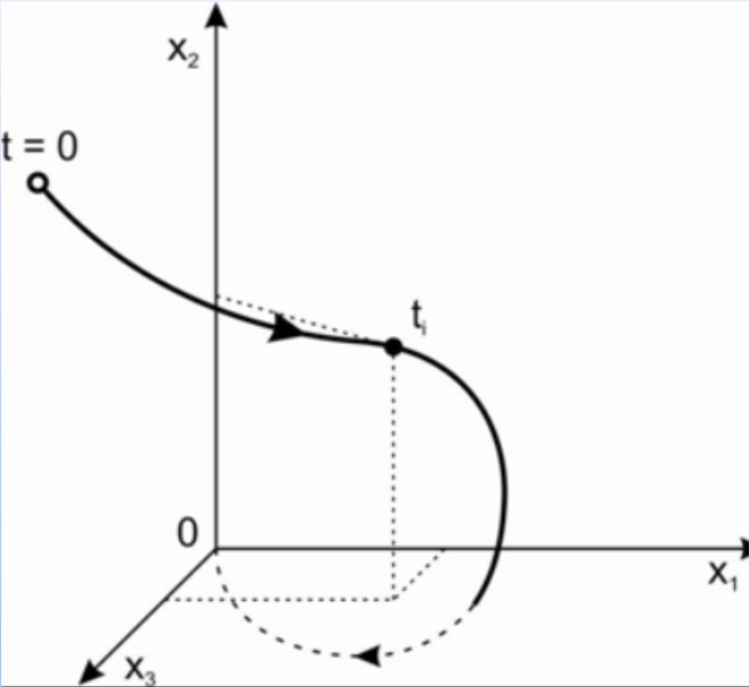
\includegraphics[width=5cm]{IMAGENES/estados}
        \caption{Espacio de Estados.}
\end{figure}
\subsection{Ejemplos}
\begin{itemize}
    \item Sea un sistema, cuyas ecuaciones que lo modelan son $u(t)-kx(t)-b\dot{x}(t)=m\ddot{x}(t)$. Hallar su representación en variables de estado
    
    Seleccionaremos las siguientes variables de estado.
    \begin{equation}
        \begin{split}
        x_{1}&=x(t)=y(t)\\
        x_{2}&=\dot{x}(t)\\
        u_{1}&=u(t)\\
        \label{eq:state_ejem1}
        \end{split}
    \end{equation}
    Reemplazando estas variables en la ecuación Dadas
    \begin{equation}
        \begin{split}
        \dot{x_{1}}&=x_{2}(t)\\
        \dot{x_{2}}&=\frac{-k}{m}x_{1}(t)+\frac{-b}{m}x_{2}(t)+\frac{1}{m}u_{1}(t)\\
        y(t)&=x_{1}\\
        \label{eq:state_ejem11}
        \end{split}
    \end{equation}
    En forma matricial se tendrá
    \begin{equation}
        \begin{split}
            \begin{bmatrix}
                \dot{x_{1}} \\
                \dot{x_{2}} \\
            \end{bmatrix}&=
            \begin{bmatrix}
                0 & 1 \\
                \frac{-k}{m} & \frac{-b}{m} \\
            \end{bmatrix}
            \begin{bmatrix}
                x_{1} \\
                x_{2} \\
            \end{bmatrix}+
            \begin{bmatrix}
                0 \\
                \frac{1}{m} \\
            \end{bmatrix}u_{1}\\
            y&=
            \begin{bmatrix}
                1 & 0\\
            \end{bmatrix}
            \begin{bmatrix}
                x_{1} \\
                x_{2} \\
            \end{bmatrix}\\
        \label{eq:state_ejem12}
        \end{split}
    \end{equation}

    \item Sea un sistema, cuyas ecuaciones que lo modelan son $m_{1}\ddot{y_{1}}+b\dot{y_{1}}+k(y_{1}-y_{2})=0$ y $m_{2}\ddot{y_{2}}+k(y_{2}-y_{1})=u$. Hallar su representación en variables de estado
    
    Seleccionaremos las siguientes variables de estado.
    \begin{equation}
        \begin{split}
        x_{1}&=y_{1}\\
        x_{2}&=\dot{y_{1}}\\
        x_{3}&=y_{2}\\
        x_{4}&=\dot{y_{2}}\\
        \label{eq:state_ejem2}
        \end{split}
    \end{equation}

    Reemplazando estas variables en la ecuación Dadas
    \begin{equation}
        \begin{split}
        \dot{x_{1}}&=x_{2}\\
        \dot{x_{2}}&=\frac{1}{m_{1}}(-b\dot{y_{1}}-k(y_{1}-y_{2}))\\
        \dot{x_{3}}&=x_{4}\\
        \dot{x_{4}}&=\frac{1}{m_{2}}(-k(y_{2}-y_{1})+u)\\
        \label{eq:state_ejem21}
        \end{split}
    \end{equation}

    En forma matricial se tendrá
    \begin{equation}
        \begin{split}
            \begin{bmatrix}
                \dot{x_{1}} \\
                \dot{x_{2}} \\
                \dot{x_{3}} \\
                \dot{x_{4}} \\
            \end{bmatrix}&=
            \begin{bmatrix}
                0 & 1 & 0 & 0\\
                \frac{-k}{m_{1}} & \frac{-b}{m_{1}} & \frac{k}{m_{1}} & 0\\
                0 & 0 & 0 & 1\\
                \frac{k}{m_{2}} & 0 & \frac{-k}{m_{2}} & 0\\
            \end{bmatrix}
            \begin{bmatrix}
                x_{1} \\
                x_{2} \\
                x_{3} \\
                x_{4} \\
            \end{bmatrix}+
            \begin{bmatrix}
                0 \\
                0 \\
                0 \\
                \frac{1}{m_{2}} \\
            \end{bmatrix}u\\
            y&=
            \begin{bmatrix}
                1 & 0 & 0 & 0\\
                0 & 0 & 1 & 0\\
            \end{bmatrix}
            \begin{bmatrix}
                x_{1} \\
                x_{2} \\
                x_{3} \\
                x_{4} \\
            \end{bmatrix}\\
        \label{eq:state_ejem22}
        \end{split}
    \end{equation}

    \item Sea un sistema, cuyas ecuaciones que lo modelan son $i_(c)=C\frac{dv_{c}}{dt}=u(t)-i_{L}$ , $L\frac{di_{L}}{dt}=-Ri_{L}+v_{c}$ y $v_{o}=Ri_{L}$. 
    
    Hallar su representación en variables de estado

    Seleccionaremos las siguientes variables de estado.
    \begin{equation}
        \begin{split}
        x_{1}&=v_{c}\\
        x_{2}&=i_{L}\\
        y&=v_{o}\\
        \label{eq:state_ejem3}
        \end{split}
    \end{equation}

    Reemplazando estas variables en la ecuación Dadas
    \begin{equation}
        \begin{split}
        \dot{x_{1}}&=\frac{-1}{C}x_{2}+\frac{1}{C}u\\
        \dot{x_{2}}&=\frac{1}{L}x_{1}+\frac{-R}{L}x_{2}
        \label{eq:state_ejem31}
        \end{split}
    \end{equation}
    En forma matricial se tendrá
    \begin{equation}
        \begin{split}
            \begin{bmatrix}
                \dot{x_{1}} \\
                \dot{x_{2}} \\
            \end{bmatrix}&=
            \begin{bmatrix}
                0 & \frac{-1}{C} \\
                \frac{1}{L} & \frac{-R}{L}\\
            \end{bmatrix}
            \begin{bmatrix}
                x_{1} \\
                x_{2} \\
            \end{bmatrix}+
            \begin{bmatrix}
                \frac{1}{C} \\
                0 \\
            \end{bmatrix}u\\
            y&=
            \begin{bmatrix}
                0 & R \\
            \end{bmatrix}
            \begin{bmatrix}
                x_{1} \\
                x_{2} \\
            \end{bmatrix}\\
        \label{eq:state_ejem32}
        \end{split}
    \end{equation}

    \item Sea un sistema, cuyas ecuaciones que lo modelan son $\frac{d^3y(t)}{dt^3}+5\frac{d^2y(t)}{dt^2}+3\frac{dy(t)}{dt}+y(t)+\int_{0}^{t} y(\tau)d\tau=r(\tau)$. 
    Hallar su representación en variables de estado

    Seleccionaremos las siguientes variables de estado.
    \begin{equation}
        \begin{split}
        x_{1}&=\int_{0}^{t} y(\tau)d\tau\\
        x_{2}&=\dot{x_{1}}\\
        x_{3}&=\dot{y}\\
        x_{4}&=\ddot{y}\\
        \label{eq:state_ejem4}
        \end{split}
    \end{equation}

    En forma matricial se tendrá
    \begin{equation}
        \begin{split}
            \begin{bmatrix}
                \dot{x_{1}} \\
                \dot{x_{2}} \\
                \dot{x_{3}} \\
                \dot{x_{4}} \\
            \end{bmatrix}&=
            \begin{bmatrix}
                0 & 1 & 0 & 0\\
                0 & 0 & 1 & 0\\
                0 & 0 & 0 & 1\\
                -1 & -1 & -3 & -5\\
            \end{bmatrix}
            \begin{bmatrix}
                x_{1} \\
                x_{2} \\
                x_{3} \\
                x_{4} \\
            \end{bmatrix}+
            \begin{bmatrix}
                0 \\
                0 \\
                0 \\
                1 \\
            \end{bmatrix}u\\
            y&=
            \begin{bmatrix}
                1 & 0 & 0 & 0\\
            \end{bmatrix}
            \begin{bmatrix}
                x_{1} \\
                x_{2} \\
                x_{3} \\
                x_{4} \\
            \end{bmatrix}\\
        \label{eq:state_ejem42}
        \end{split}
    \end{equation}

\end{itemize}
\section{Criterio de Controlabilidad y Observabilidad}
\textbf{Criterio de Controlabilidad:}
\vspace{5mm}

Un sistema es completamente controlable si todas las variables de estado del proceso pueden ser controladas para alcanzar un determinado objetivo en un tiempo finito por un control sin restricciones $u(t)$, si alguna de las variables de estado no depende de $u(t)$ entonces se dice que esta variable es incontrolable, y en el caso esto suceda, se dice que el sistema no es completamente controlable. La controlabilidad puede ser definida tambien para las salidas del sistema, asi que se debe diferenciar entre controlabilidad de estados y controlabilidad del sistema.

Se dice que el estado $x(t)$ es controlable en $t=t_{0}$ si existe una entrada $u(t)$ que llevará el estado a cualquier estado final $x(t_{1})$ por un tiempo finito.

Sea las siguientes definiciones
\begin{equation}
    \begin{split}
        e^{A(t-\tau)}&=\displaystyle\sum_{i=0}^{}\,\gamma_{i}A^i\\
        x&=\int_{0}^{t}e^{A(t-\tau)}Bu d\tau=\displaystyle\sum_{i=0}^{}\,\gamma_{i}(t-\tau)A^iBu d\tau\\
        \rho_{i}&=\int\gamma_{i}u(\tau)d\tau
        x(t)=\displaystyle\sum_{i=0}^{}\,A^iB\rho_{t}=
        \begin{bmatrix}
            B & AB & ... & A^{n-1}B \\
        \end{bmatrix}
        \begin{bmatrix}
            \rho_{1}(t) \\
            : \\
            : \\
            \rho_{4}(t) \\
        \end{bmatrix}\\
        \label{eq:obs_demos}
    \end{split}
\end{equation}

La matriz de controlabilidad estará dada por 
\begin{equation}
    \begin{split}
        \begin{bmatrix}
            B & AB & ... & A^{n-1}B \\
        \end{bmatrix}
        \label{eq:matriz_control}
    \end{split}
\end{equation}

El sistema será controlable solo si esta matriz es de rango máximo.
\vspace{5mm}
\textbf{Criterio de Observabilidad:}
\vspace{5mm}
Dado un sistema LTI descrito por ecuaciones dinámicas, un estado $x(t)$ es observable si para una entrada $u(t)$, existe un tiempo finito $t_{f}\geq t_{0}$ , tal que, conociendo $u(t)$ para $t_{0}\leq t<t_{f}$ y las matrices A,B,C y D y la salida $y(t)$ para en intervalo $t_{0}\leq t<t_{f}$ sean suficientes para determinar $x(t_{0})$. Si todos los estados de un sistema son observables para un tiempo finito $t_{f}$ se puede decir que el sistema es completamente observable.

Sea la matriz de Observabilidad 
\begin{equation}
    \begin{split}
        \begin{bmatrix}
            C \\
            CA \\
            CA^2 \\
            : \\
            : \\
            CA^{n-1} \\
        \end{bmatrix}
        \label{eq:matriz_observ}
    \end{split}
\end{equation}
Si esta matriz es de rango completo el sistema es observable.
\subsection{Ejemplos}
\begin{itemize}
    \item Determinar si el siguiente sistema es controlable
    \begin{equation}
        \begin{split}
            A&=
            \begin{bmatrix}
                1 & 2 \\
                1 & 0 \\
            \end{bmatrix}
            B=
            \begin{bmatrix}
                -2 \\
                3 \\
            \end{bmatrix}\\
            \begin{bmatrix}
                B & AB & ... & A^{n-1}B \\
            \end{bmatrix}&=
            \begin{bmatrix}
                -2 & 4 \\
                3 & -2 \\
            \end{bmatrix}
        \end{split}
        \label{eq:controla1}
    \end{equation}

    El sistema es controlable

    \item Determinar si el siguiente sistema  es controlable
    \begin{equation}
        \begin{split}
            A&=
            \begin{bmatrix}
                2 & 1 & 3 \\
                3 & 1 & 4 \\
                1 & 0 & 1 \\
            \end{bmatrix}
            B=
            \begin{bmatrix}
                1 \\
                2 \\
                0 \\
            \end{bmatrix}\\
            \begin{bmatrix}
                B & AB & ... & A^{n-1}B \\
            \end{bmatrix}&=
            \begin{bmatrix}
                1 & 4 & 16 \\
                2 & 5 & 21 \\
                0 & 1 & 5 \\
            \end{bmatrix}
        \end{split}
        \label{eq:controla1}
    \end{equation}

    El sistema es controlable

    \item Determinar si el siguiente sistema es observable
    \begin{equation}
        \begin{split}
            A&=
            \begin{bmatrix}
                1 & 2 \\
                1 & 0 \\
            \end{bmatrix}
            B=
            \begin{bmatrix}
                -2 \\
                3 \\
            \end{bmatrix}\\
            C=
            \begin{bmatrix}
                1 & 0\\
            \end{bmatrix}\\
            \begin{bmatrix}
                C \\
                CA \\
            \end{bmatrix}&=
            \begin{bmatrix}
                1 & 0 \\
                1 & 2 \\
            \end{bmatrix}
        \end{split}
        \label{eq:controla1}
    \end{equation}

    El sistema es observable

    \item Determinar si el siguiente sistema es observable
    \begin{equation}
        \begin{split}
            A&=
            \begin{bmatrix}
                2 & 1 & 3 \\
                3 & 1 & 4 \\
                1 & 0 & 1 \\
            \end{bmatrix}
            B=
            \begin{bmatrix}
                1 \\
                2 \\
                0 \\
            \end{bmatrix}
            C=
            \begin{bmatrix}
                1 & 0 & 1\\
            \end{bmatrix}\\
            \begin{bmatrix}
                C \\
                CA \\
                CA^2 \\
            \end{bmatrix}&=
            \begin{bmatrix}
                1 & 0 & 1 \\
                3 & 1 & 4 \\
                13 & 4 & 17 \\
            \end{bmatrix}
        \end{split}
        \label{eq:controla1}
    \end{equation}

    El sistema no es observable
\end{itemize}

\section{Solución de Sistema de Ecuaciones Mediante la Función de Transferencia}
Usaremos la transformada inversa de Laplace para solucionar el sistema de ecuaciones mediante la función de transferencia.
\subsection{Ejemplos}
\begin{itemize}
    \item Sea la siguiente función de transferencia $\frac{Y(s)}{R(s)}=\frac{5}{s^3+10s^2+200s}$ determinar su respuesta a una entrada de escalon unitario $R(s)=\frac{1}{s}$.
    
    La respuesta del sistema estará dada por 
    \begin{equation}
        \begin{split}
            Y(s)&=\frac{5}{s(s^3+10s^2+200s)}\\
            \label{eq:inverse_laplace1}
        \end{split}
    \end{equation}
    Desarrollando por fracciones parciales, la ecuación \ref{eq:inverse_laplace1} se expresara como
    \begin{equation}
        \begin{split}
            Y(s)&=\frac{-1}{800s}+\frac{1}{40s^2}+\frac{s\frac{1}{800}-\frac{1}{80}}{s^2+10s+200}\\
            Y(s)&=\frac{1}{40s^2}+\frac{-1}{800s}+\frac{-3}{160}\frac{1}{(s+5)^2+175}+\frac{1}{800}\frac{s+5}{(s+5)^2+175}\\
            \label{eq:inverse_laplace11}
        \end{split}
    \end{equation}
    Tomando la transformada inversa de Laplace en la ecuación \ref{eq:inverse_laplace11} se tendrá.
    \begin{equation}
        \begin{split}
            y(t)&=\frac{t}{40}+\frac{-1}{800}+\frac{-3}{160}\frac{1}{5\sqrt(7)}e^{-5t}sen(5\sqrt(7)t)+\frac{1}{800}e^{-5t}cos(5\sqrt(7)t)\\
            \label{eq:inverse_laplace12}
        \end{split}
    \end{equation}

    \item Sea la siguiente función de transferencia $\frac{Y(s)}{R(s)}=\frac{1}{s^3+10s^2+200s}$ determinar su respuesta a una entrada de escalon unitario $R(s)=\frac{1}{s^2}$.
    
    La respuesta del sistema estará dada por 
    \begin{equation}
        \begin{split}
            Y(s)&=\frac{1}{s^2(s^3+10s^2+200s)}\\
            \label{eq:inverse_laplace2}
        \end{split}
    \end{equation}
    Desarrollando por fracciones parciales, la ecuación \ref{eq:inverse_laplace2} se expresara como
    \begin{equation}
        \begin{split}
            Y(s)&=\frac{1}{40s^3}+\frac{-1}{800s^2}+\frac{-1}{1600s}+\frac{1}{1600}\frac{s+5}{(s+5)^2+175}+\frac{1}{640}\frac{1}{(s+5)^2+175}\\
            \label{eq:inverse_laplace21}
        \end{split}
    \end{equation}
    Tomando la transformada inversa de Laplace en la ecuación \ref{eq:inverse_laplace21} se tendrá.
    \begin{equation}
        \begin{split}
            y(t)&=\frac{t^2}{80}+\frac{-1}{1600}+\frac{-t}{800}+\frac{1}{1600}e^{-5t}cos(5\sqrt(7)t)+\frac{1}{5\sqrt(7)640}e^{-5t}sen(5\sqrt(7)t)\\
            \label{eq:inverse_laplace22}
        \end{split}
    \end{equation}

    \item Sea la siguiente función de transferencia $\frac{Y(s)}{R(s)}=\frac{s}{s^2+4s+5}$ determinar su respuesta a una entrada de escalon unitario $R(s)=\frac{1}{s}$.
    
    La respuesta del sistema estará dada por 
    \begin{equation}
        \begin{split}
            Y(s)&=\frac{1}{s^2+4s+5}\\
            \label{eq:inverse_laplace3}
        \end{split}
    \end{equation}
    Desarrollando por fracciones parciales, la ecuación \ref{eq:inverse_laplace3} se expresara como
    \begin{equation}
        \begin{split}
            Y(s)&=\frac{s+2}{(s+2)^2+1}+\frac{-2}{(s+2)^2+1}\\
            \label{eq:inverse_laplace31}
        \end{split}
    \end{equation}
    Tomando la transformada inversa de Laplace en la ecuación \ref{eq:inverse_laplace31} se tendrá.
    \begin{equation}
        \begin{split}
            y(t)&=e^{-2t}cos(t)-2e^{-2t}sen(t)\\
            \label{eq:inverse_laplace32}
        \end{split}
    \end{equation}

\item Sea la siguiente función de transferencia $\frac{Y(s)}{R(s)}=\frac{1}{s^{\frac{3}{2}}}$ determinar su respuesta a una entrada de escalon unitario $R(s)=\frac{1}{s}$.
    
    La respuesta del sistema estará dada por 
    \begin{equation}
        \begin{split}
            Y(s)&=\frac{1}{s^{\frac{3}{2}}}\\
            \label{eq:inverse_laplace4}
        \end{split}
    \end{equation}
    Desarrollando para llegar a la forma $L^{-1}(\frac{(2n-1)!\sqrt{\pi}}{2^{sn+\frac{1}{2}}})$, \ref{eq:inverse_laplace4} se expresara como
    \begin{equation}
        \begin{split}
            Y(s)&=\frac{3\pi^{\frac{1}{2}}}{2^2s^{\frac{3}{2}}}\\
            \label{eq:inverse_laplace41}
        \end{split}
    \end{equation}
    Tomando la transformada inversa de Laplace en la ecuación \ref{eq:inverse_laplace41} se tendrá.
    \begin{equation}
        \begin{split}
            y(t)&=\frac{4t^{\frac{3}{2}}}{3\pi^{\frac{1}{2}}}\\
            \label{eq:inverse_laplace42}
        \end{split}
    \end{equation}
\end{itemize}
\section{Solución de las Ecuaciones de Estado}
Resolveremos las ecuaciones diferenciales de las variables de estado en el dominio del tiempo.
\subsection{Ejemplos}
\begin{itemize}
    \item Sea la siguiente ecuación diferencial que modela un sistema $\ddot{y}+4\dot{y}+y=5r(t)$ calcular la respuesta en el tiempo del sistema para $r(t)=\mu(t)$.
    La ecuación diferencial quedará
    \begin{equation}
        \begin{split}
            \ddot{y}+4\dot{y}+y&=5\\
            \label{eq:ode1}
        \end{split}
    \end{equation}
    Esta ecuación es una ODE de segundo orden con coeficientes constantes, la solución general estará dada por la ecuación característica $m^2+4m+1=0$.
    La solución particular será simplemente $5$, entonces se tendrá
    \begin{equation}
        \begin{split}
            y_{p}+y_{g}=c_{1}e^{\frac{t(-\sqrt{2}+1)}{\sqrt{2}}}+c_{2}e^{\frac{-t(\sqrt{2}+1)}{\sqrt{2}}}+5\\
            \label{eq:ode12}
        \end{split}
    \end{equation}
    Donde $c_{1}$ y $c_{2}$ dependen de las condiciones iniciales del sistema.

    \item Sea la siguiente ecuación diferencial que modela un sistema $\ddot{y}+4\dot{y}+y=r(t)$ calcular la respuesta en el tiempo del sistema para $r(t)=t$.
    La ecuación diferencial quedará
    \begin{equation}
        \begin{split}
            \ddot{y}+4\dot{y}+y&=t\\
            \label{eq:ode2}
        \end{split}
    \end{equation}
    Esta ecuación es una ODE de segundo orden con coeficientes constantes, la solución general estará dada por la ecuación característica $m^2+4m+1=0$.
    La solución particular será $t-4$, entonces se tendrá
    \begin{equation}
        \begin{split}
            y_{p}+y_{g}=c_{1}e^{\frac{t(-\sqrt{2}+1)}{\sqrt{2}}}+c_{2}e^{\frac{-t(\sqrt{2}+1)}{\sqrt{2}}}+t-4\\
            \label{eq:ode21}
        \end{split}
    \end{equation}
    Donde $c_{1}$ y $c_{2}$ dependen de las condiciones iniciales del sistema.

    \item Sea la siguiente ecuación diferencial que modela un sistema $u(t)-kx(t)-b\dot{x}(t)=m\ddot{x}(t)$ calcular la respuesta en el tiempo del sistema para $u(t)=1$ para $m=1,k=1,b=1$.
    \begin{equation}
        \begin{split}
            \ddot{x}(t)+\dot{x}(t)+x(t)&=1\\
            \label{eq:ode3}
        \end{split}
    \end{equation}
    Esta ecuación es una ODE de segundo orden con coeficientes constantes, la solución general estará dada por la ecuación característica $m^2+m+1=0$.
    La solución particular será $1$, entonces se tendrá
    \begin{equation}
        \begin{split}
            y_{p}+y_{g}=e^{\frac{-t}{2}}(c_{1}cos(\frac{\sqrt{3}t}{2})+c_{2}sen(\frac{\sqrt{3}t}{2}))+1\\
            \label{eq:ode31}
        \end{split}
    \end{equation}
    Donde $c_{1}$ y $c_{2}$ dependen de las condiciones iniciales del sistema.

    \item Sea la siguiente ecuación diferencial que modela un sistema $u(t)-kx(t)-b\dot{x}(t)=m\ddot{x}(t)$ calcular la respuesta en el tiempo del sistema para $u(t)=t$ para $m=1,k=1,b=1$.
    \begin{equation}
        \begin{split}
            \ddot{x}(t)+\dot{x}(t)+x(t)&=t\\
            \label{eq:ode4}
        \end{split}
    \end{equation}
    Esta ecuación es una ODE de segundo orden con coeficientes constantes, la solución general estará dada por la ecuación característica $m^2+m+1=0$.
    La solución particular será $t-1$, entonces se tendrá
    \begin{equation}
        \begin{split}
            y_{p}+y_{g}=e^{\frac{-t}{2}}(c_{1}cos(\frac{\sqrt{3}t}{2})+c_{2}sen(\frac{\sqrt{3}t}{2}))+t-1\\
            \label{eq:ode41}
        \end{split}
    \end{equation}
    Donde $c_{1}$ y $c_{2}$ dependen de las condiciones iniciales del sistema.
\end{itemize}
\section{Lugar Geométrico de las Raices}
Es un metodo gráfico para examinar el comportamiento de las raices de un sistema frente a la variación de algun parametro en lazo cerrado. Nos permite a determinar la estabilidad del sistema. 

Sea el sistema en lazo cerrado
\begin{equation}
    \begin{split}
        \frac{Y(s)}{X(s)}&=\frac{G(s)}{1+H(s)G(s)}\\
        \label{eq:root}
    \end{split}
\end{equation}

Podemos escribir el denominador $1+ H(s)G(s)$ como sigue
\begin{equation}
    \begin{split}
        0&=1+K\frac{(s-z_{1})(s-z_{2})(s-z_{3})...(s-z_{m})}{(s-p_{1})(s-p_{2})(s-p_{3})...(s-p_{n})}\\
        \label{eq:root1}
    \end{split}
\end{equation}

Los lugares de las raíces para el sistema son los lugares de los polos en lazo cerrado cuando la ganancia K varía de cero a infinito. \cite{ogata2003ingenieria} 
\subsection{Ejemplos}
\begin{itemize}
    \item Graficar el lugar de las raices para $\frac{1}{s(s^2+5s+6)}$
    
    Observando la función de transferencia, podemos ver que tiene infitos ceros, y 3 polos en $s=0,-3,-2$

    Podemos reescribir la función de transferencia en lazo abierto como $G(s)H(s)=\frac{N(s)}{D(s)}$ de aqui tendremos que $N(s)= 1$ y $D(s)= s^3+5s^2 +6s$
    
    La ecuación característica será $D(s)+KN(s)=s^3+5s^2+6s+K = 0$
    
    \begin{figure}[h]
        \centering
            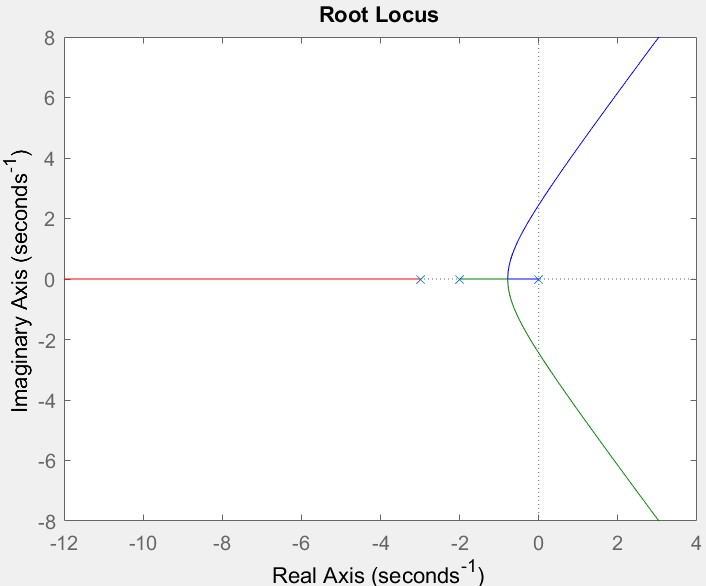
\includegraphics[width=8cm]{IMAGENES/locus1}
            \caption{Ejemplo 1}
    \end{figure}
    
    \item Graficar el lugar de las raices para $\frac{s+3}{s(s^2-s-2)}$
    \lstinputlisting[language=Matlab]{Matlab/lugar_raices2.m}
    \begin{figure}[h]
        \centering
            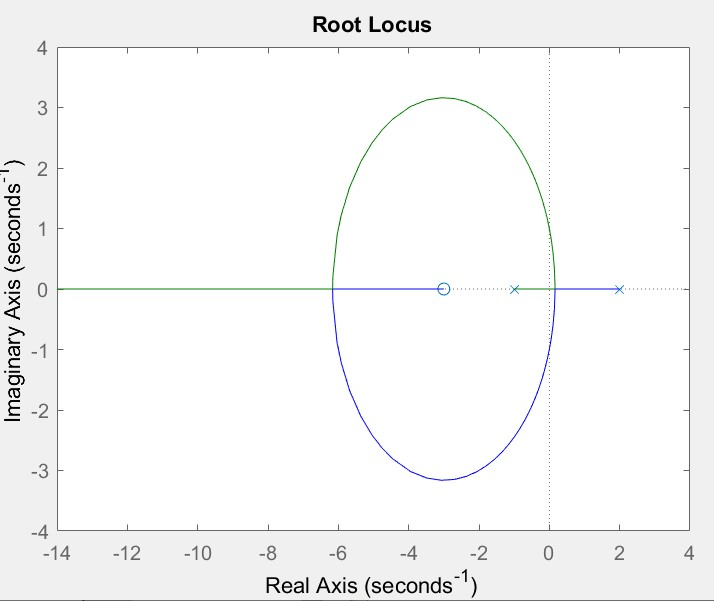
\includegraphics[width=8cm]{IMAGENES/locus2}
            \caption{Ejemplo 2}
    \end{figure}

    \item Graficar el lugar de las raices para $\frac{s+1}{s^3+4s^2+6s+4}$
    \lstinputlisting[language=Matlab]{Matlab/lugar_raices3.m}
    \begin{figure}[h]
        \centering
            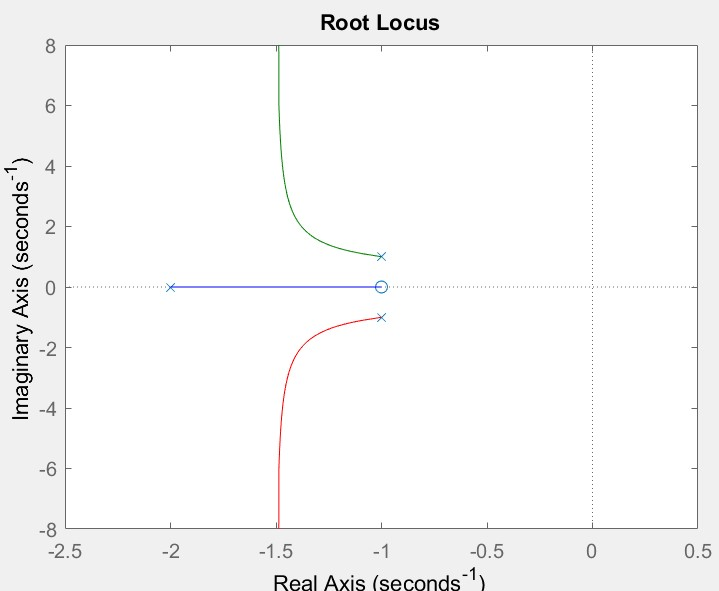
\includegraphics[width=8cm]{IMAGENES/locus3}
            \caption{Ejemplo 3}
    \end{figure}

    \item Graficar el lugar de las raices para $\frac{s^2+2s+2}{s^4+9s^3+33s^2+51s^2+26s}$
    \lstinputlisting[language=Matlab]{Matlab/lugar_raices4.m}
    \begin{figure}[h]
        \centering
            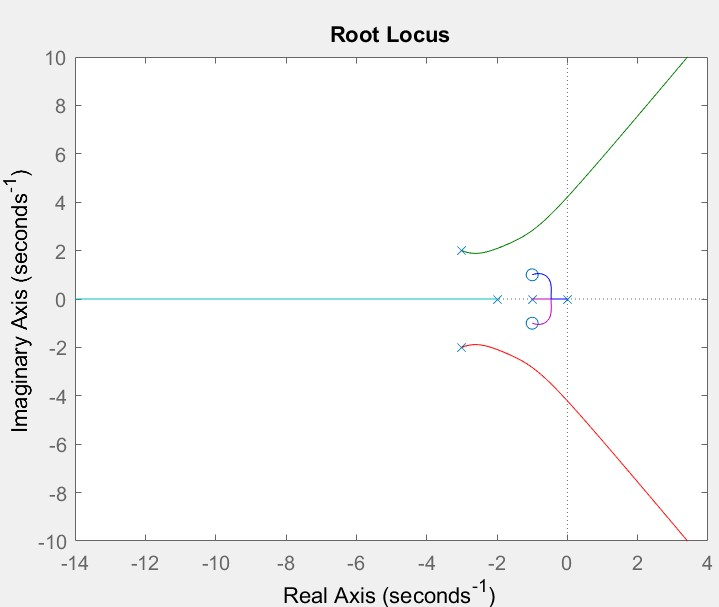
\includegraphics[width=8cm]{IMAGENES/locus4}
            \caption{Ejemplo 4}
    \end{figure}
\end{itemize}

\section{Metodos para la Asignación de Polos para el Diseño de Controladores}
La fórmula de Ackermann es un metodo de diseño para resolver este problema de asignación de polos para sistemas LTI, con este metodo se puede hacer el diseño en un solo paso para sistemas representados en espacio de estados.
Consiste en calcular una nueva ganancia en lazo cerrado $K$, esta se calculará usando la siguiente fórmula.
\begin{equation}
    \begin{split}
        K=
        \begin{bmatrix}
            0 & 0 & ... & 1\\
        \end{bmatrix}
        M^{-1}_{c}p_{c}(A)
    \end{split}
    \label{eq:ackermann}
\end{equation}
Donde 
\begin{itemize}
    \item $M^{-1}_{c}$ es la inversa de la matriz de controlabilidad
    \item $p_{c}$ es el polinomio que contiene los polos en lazo cerrado que se desean incluir en el sistema.
    \begin{equation}
        \begin{split}
            p_{c}=S^{n}+a_{n-1}S^{n-1}+a_{n-2}S^{n-2}+...+a_{1}S+a_{0}
        \end{split}
        \label{eq:polo_closed_loop}
    \end{equation} 
\end{itemize}

\subsection{Ejemplos}
\begin{itemize}
    \item Dadas las siguientes matrices de un sistema en espacio de estados $A,B,C$ calcular la ganancia en lazo cerrado $K$ para posicionar los polos en lazo cerrado en $-1$ y $-2$
    \begin{equation}
        \begin{split}
            A=
            \begin{bmatrix}
                -1 & -2 \\
                1 & -0.4
            \end{bmatrix}
            B=
            \begin{bmatrix}
                1 \\
                -2
            \end{bmatrix}
            C=
            \begin{bmatrix}
                3 & 4 \\
            \end{bmatrix}
        \end{split}
        \label{eq:ackermann_ejem1}
    \end{equation}

    Solución

    Se desea posicionar los polos en $-1$ y $-2$ entonces se tendrá 
    \begin{equation}
        \begin{split}
            p_{c}&=(S+1)(S+2)\\
            p_{c}&=S^{2}+3S+2\\
            p_{c}(A)&=
            \begin{bmatrix}
                -1 & -2 \\
                1 & -0.4
            \end{bmatrix}^2
            +3\begin{bmatrix}
                -1 & -2 \\
                1 & -0.4
            \end{bmatrix}
            +2\begin{bmatrix}
                1 & 0 \\
                0 & 1
            \end{bmatrix}\\
            p_{c}(A)&=
            \begin{bmatrix}
                -1 & -1 \\
                -1.4 & -1.84
            \end{bmatrix}
            +3\begin{bmatrix}
                -1 & -2 \\
                1 & -0.4
            \end{bmatrix}
            +2\begin{bmatrix}
                1 & 0 \\
                0 & 1
            \end{bmatrix}\\
            p_{c}(A)&=
            \begin{bmatrix}
                -2 & -3.2 \\
                1.6 & -1.04
            \end{bmatrix}
        \end{split}
        \label{eq:polo_ejem1}
    \end{equation}
    La inversa de la matriz de controlabilidad será
    \begin{equation}
        \begin{split}
            M_{c}=
            \begin{bmatrix}
                B & AB \\
            \end{bmatrix}\\
            M_{c}=
            \begin{bmatrix}
                1 & 3 \\
                -2 & 1.8
            \end{bmatrix}\\
            M^{-1}_{c}=\frac{1}{7.8}
            \begin{bmatrix}
                1.8 & -3 \\
                2 & 1
            \end{bmatrix}\\
        \end{split}
        \label{eq:ackermann1_ejem1}
    \end{equation}
    Reemplazando \ref{eq:ackermann1_ejem1} y \ref{eq:polo_ejem1} en la fórmula de Ackermann y operando, se tendrá finalmente.
    \begin{equation}
        \begin{split}
            K=
            \begin{bmatrix}
                0 & 1 \\
            \end{bmatrix}
            M^{-1}_{c}p_{c}(A)
            =
            \begin{bmatrix}
                -0.31 & -0.95 \\
            \end{bmatrix}
        \end{split}
        \label{eq:ackermann_ejem1_result}
    \end{equation}


\end{itemize}
%$$\mathscr{L}\{f(t)\}=F(s)$$
%$$\mathscr{Z}\{f(t)\}=F(s)$$
%\begin{figure}[h]
%    \centering
%        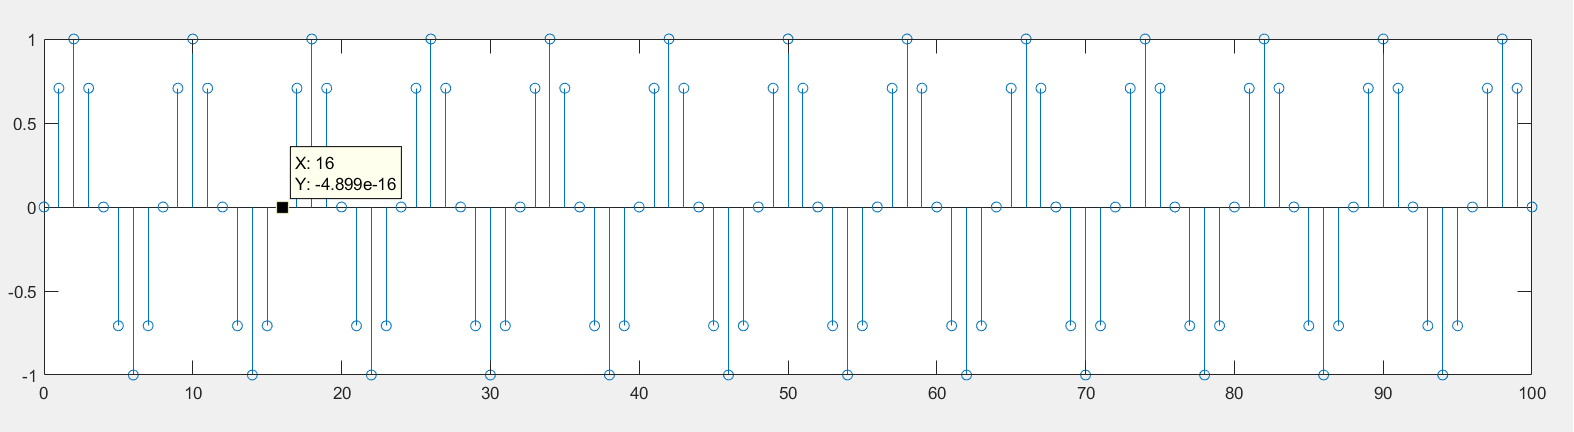
\includegraphics[width=15cm]{IMAGENES/T1_val1.png}
%        \caption{Valor de la muestra 16 para y1.}
%\end{figure}
\bibliographystyle{apacite}
\bibliography{biblio}
\end{document}